\documentclass{article}
\usepackage[utf8]{inputenc}
\usepackage{graphicx}
\usepackage{float}
\usepackage{listings}
\usepackage{fontspec}
\usepackage{gensymb}
\usepackage{amsmath}

% \setromanfont{Times New Roman}
% \setsansfont{Arial}
\setmonofont{Cousine}
\lstset{basicstyle=\footnotesize\ttfamily}

\title{HW1-Gandarillas-Victor\\
MAE 290A}
\author{Victor Gandarillas}
\date{4 November 2019}

% Discuss both tensegrity structures in your HW1report, specifically including the following for each:
% A) Is this structure potentially inconsistent?  What does that mean?
% B) is this structure undetermined?  What does that mean?  If it is underdetermined, is it pretensionable, or only tensionable under load?  Discuss.
% Also include any other salient points regarding these designs.  You are encouraged to explore well beyond the specific questions asked; extra credit will be granted as appropriate...
\begin{document}

\maketitle

\section{P1}

We construct a Michell Truss from Michell Spirals according to Figure 4.6 of \cite{skelton}.
The Michell Spirals are of order $q\in\{0,1,2,3,4\}$.
Figure \ref{fig:mt} shows a Michell Truss with a tip load (pink arrow) with bars shown in red and strings shown in blue.
The fixed nodes are shown as red triangles and the reaction forces at the fixed nodes due to the applied external load are shown as blue arrows.
Listing \ref{lst:p1} shows that all the bars are in compression and all the strings are in tension.
This is favorable since strings cannot support compression, but are much lighter than bars.

\begin{figure}[H]
  \centering
  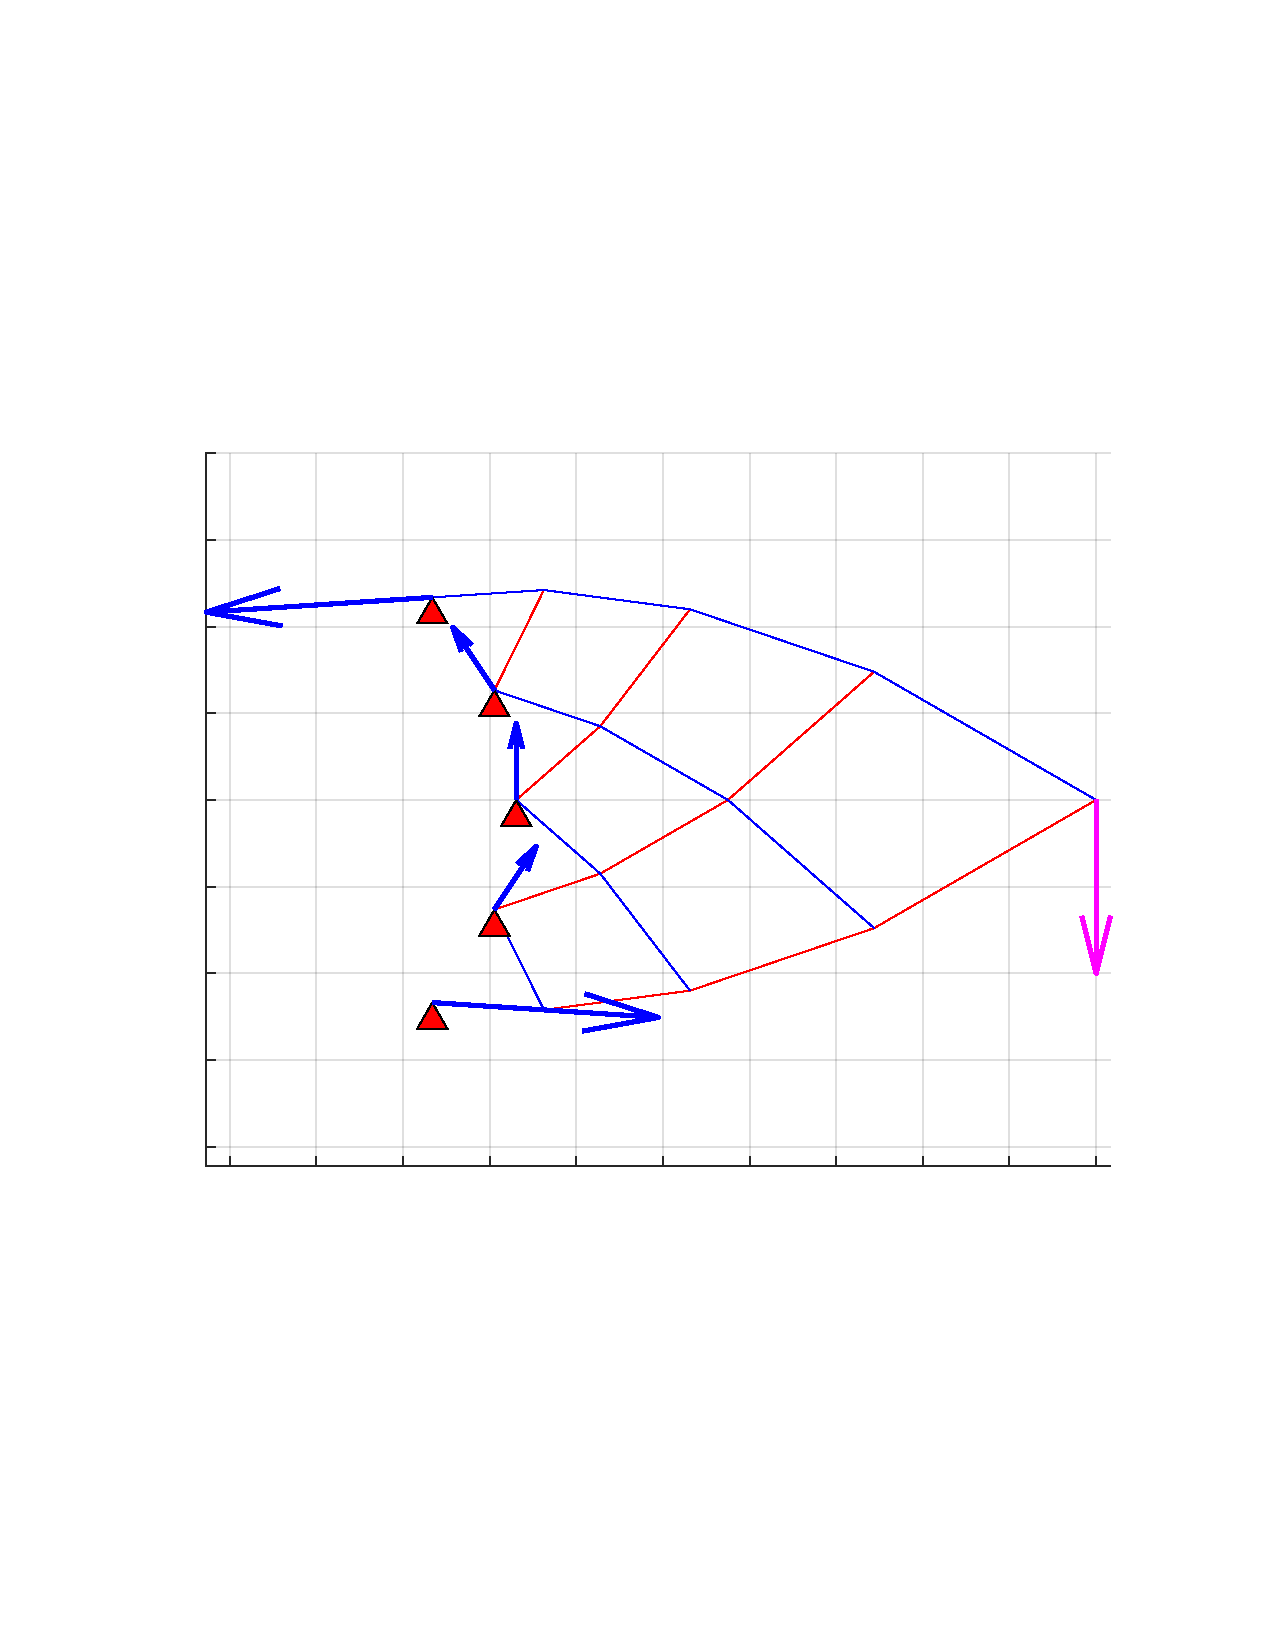
\includegraphics[clip, trim=3.5cm 7.5cm 2.5cm 7.5cm, width=0.6\textwidth]{images/michell_tip_load.pdf}
  \caption{Michell Truss with nodes defined using Michell Spirals of order 0-4 and tip load (pink arrow); bars shown in red, strings shown in blue; reaction forces at fixed nodes (red triangles) shown as blue arrows}
  \label{fig:mt}
\end{figure}

As Listing \ref{lst:p1} shows, the Michell Truss is not potentially inconsistent.
The system is also not underdetermined.
Since the system is not potentially inconsistent or underdetermined, the solution given in Listing \ref{lst:p1} corresponding to the truss in Figure \ref{fig:mt} is unique for a given load.
The fact that the system is not potentially inconsistent implies that there exists a solution for all loads.
That is, all the loads are in the column space of $A_{se}$.



\section{P2}

The regular minimal prism with 3 bars shown in Figure 3.43 of \cite{skelton} is reproduced in Figure \ref{fig:m3}.
For comparison, the top view of the regular nonminimal prism with 4 bars is shown in Figure \ref{fig:np_top}.

\begin{figure}[H]
  \centering
  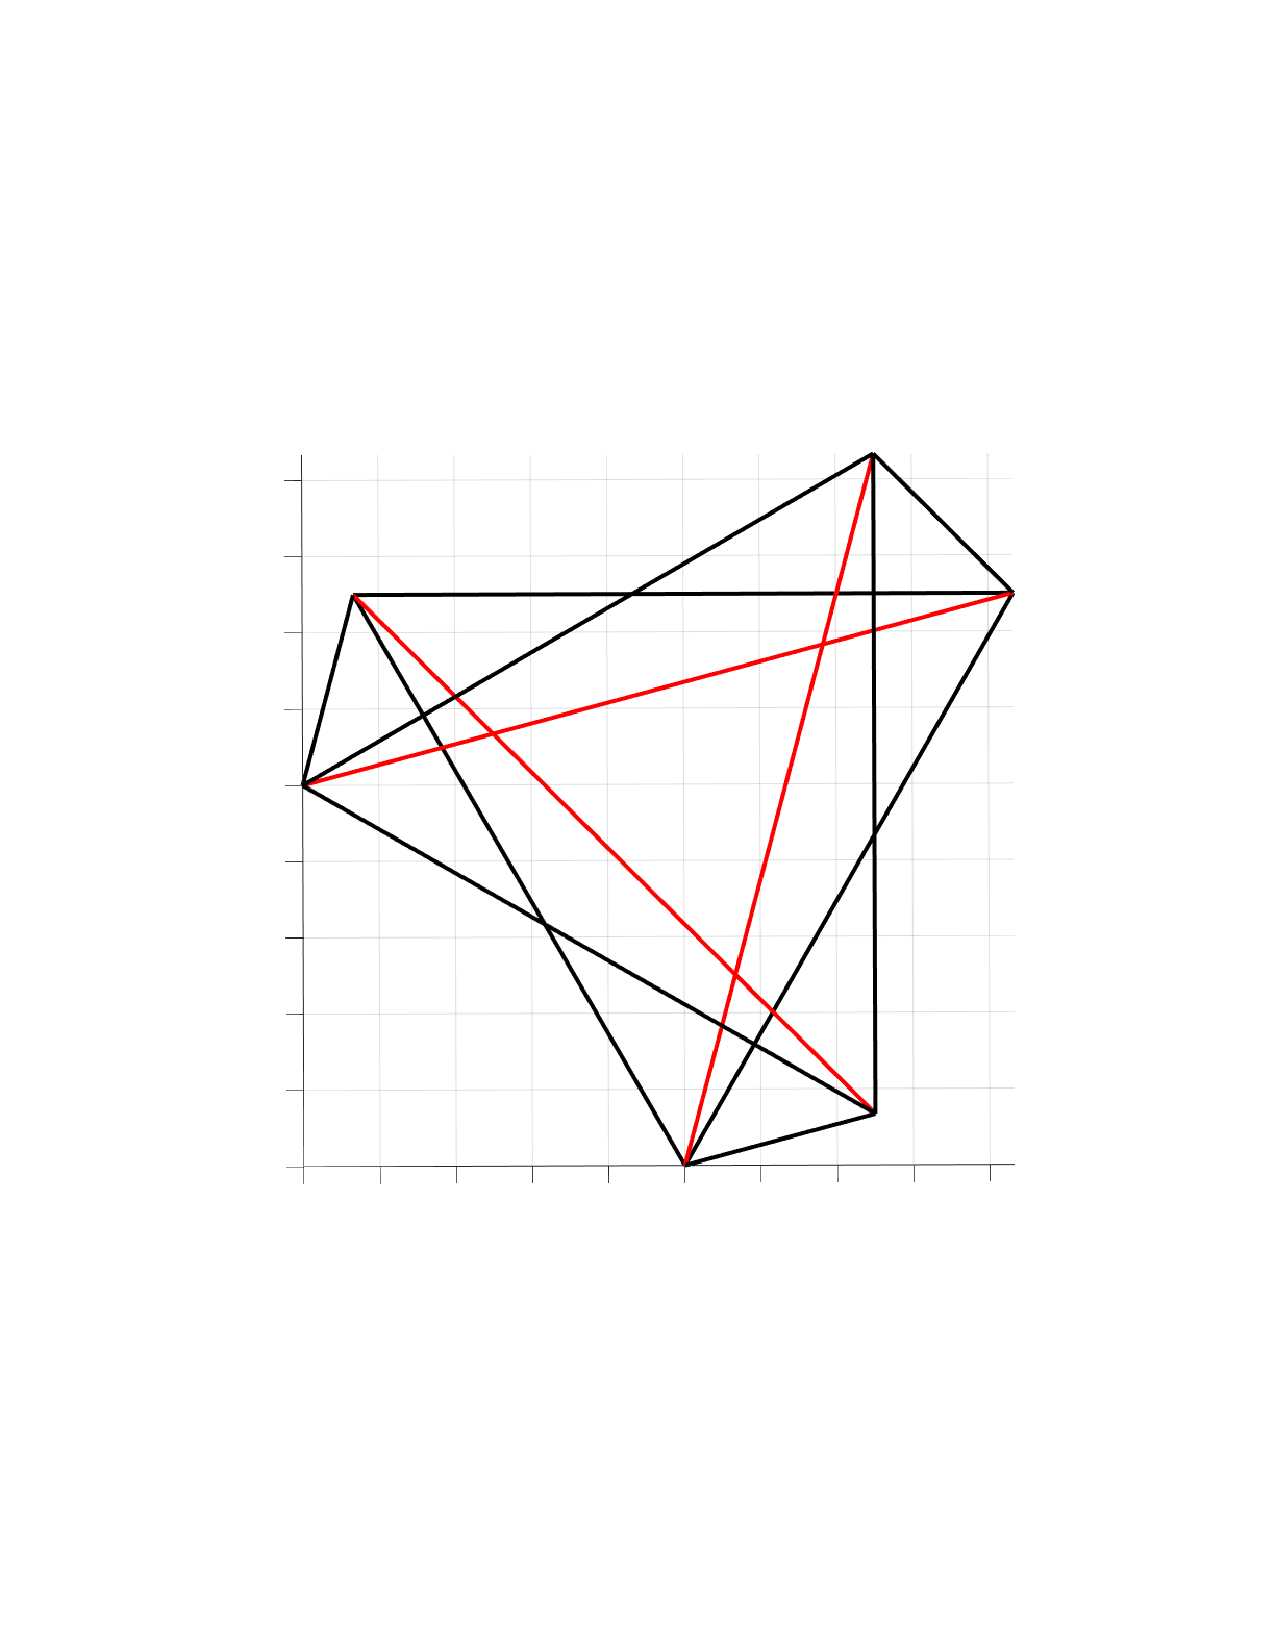
\includegraphics[clip, trim=3.5cm 7.5cm 2.5cm 7.5cm, width=0.6\textwidth]{images/minimal_prism_3.pdf}
  \caption{Top view of regular minimal prism with 3 bars and 9 strings; bars shown in red, strings shown in black}
  \label{fig:m3}
\end{figure}

\begin{figure}[H]
  \centering
  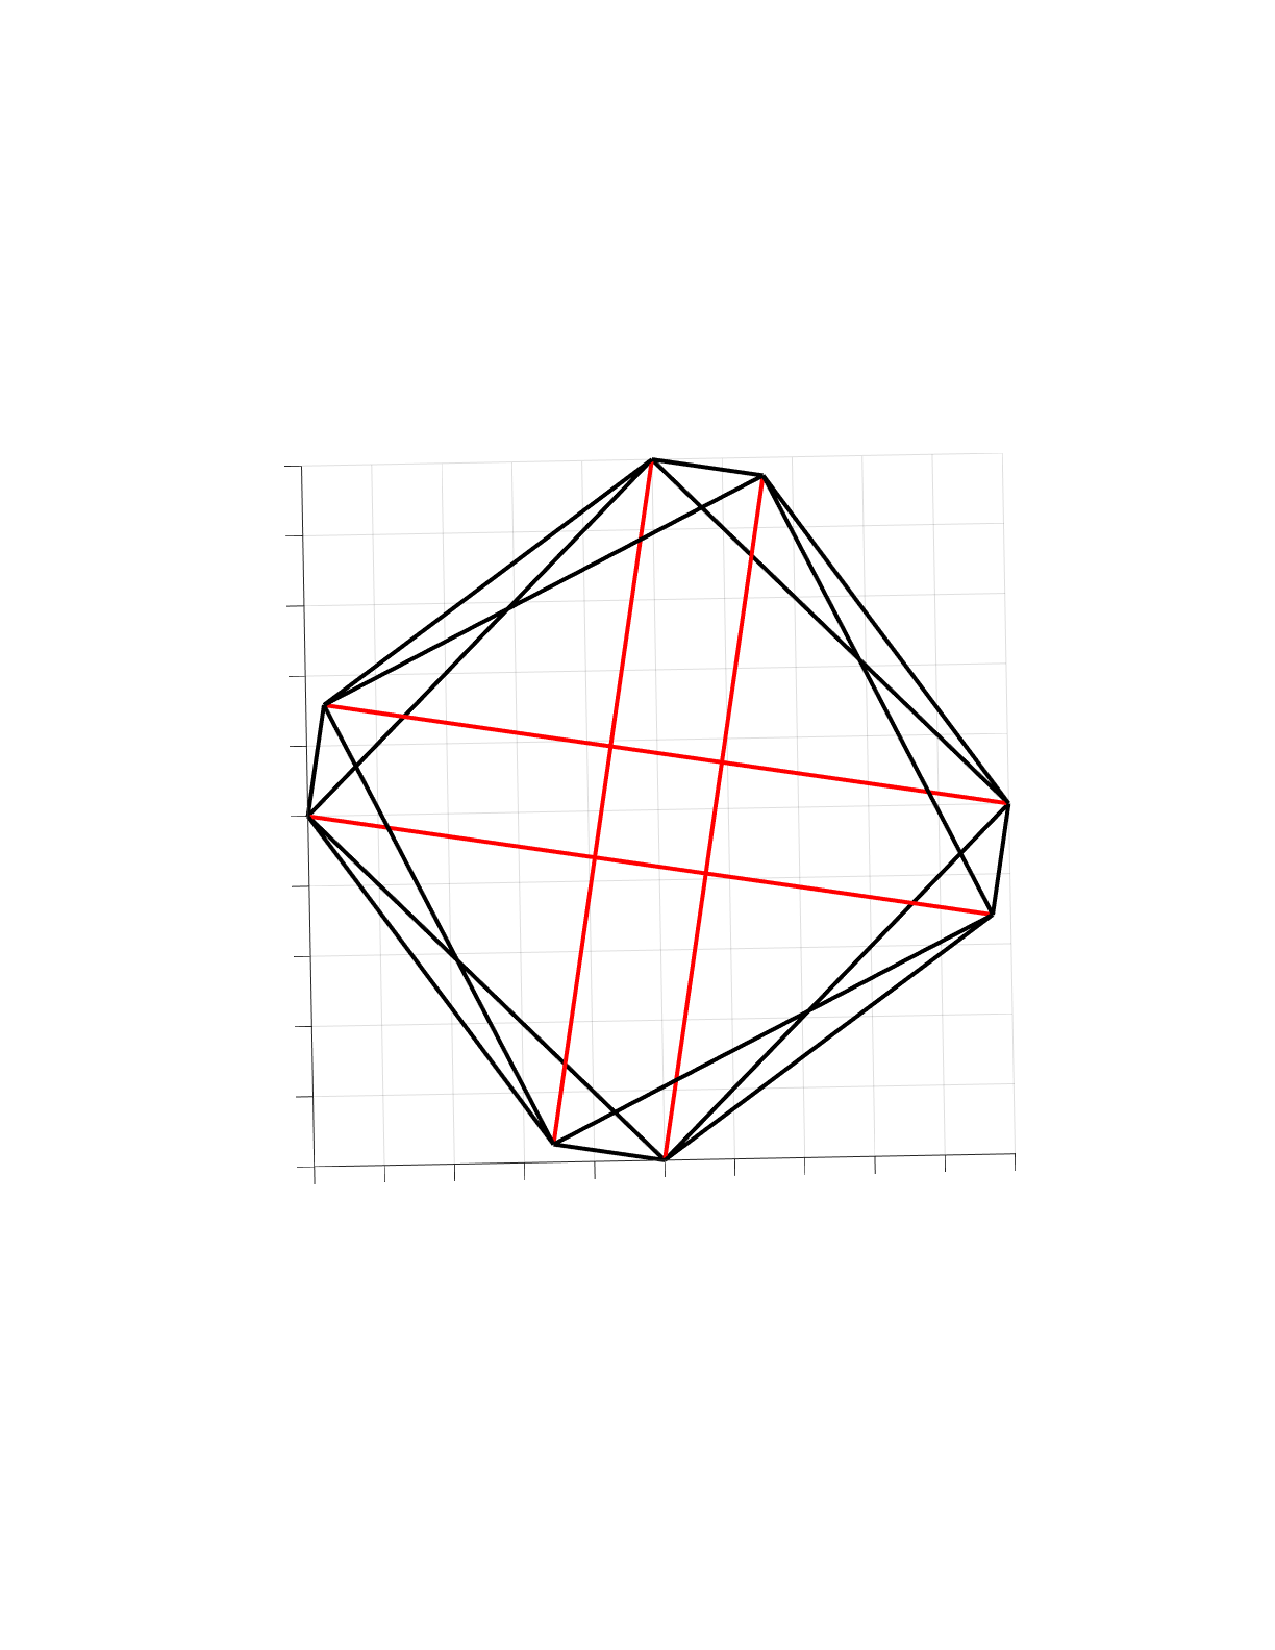
\includegraphics[clip, trim=3.5cm 7.5cm 2.5cm 7.5cm, width=0.6\textwidth]{images/nonminimal_prism_4_top.pdf}
  \caption{Top view of regular nonminimal prism with 4 bars and 16 strings; bars shown in red, strings shown in black}
  \label{fig:np_top}
\end{figure}

The default perspective view of the regular nonminimal prism with 4 bars is shown in Figure \ref{fig:np}.
The twist angle $\alpha$ is selected so that the vertical loads $\gamma_v$ and the diagonal loads $\gamma_d$ are equal.
From Equation 3.66 of \cite{skelton}, in order for $\gamma_d = \gamma_v$,

\begin{align*}
2 \cos{\alpha}\cos{\frac{\pi}{p}} &= -\cos{\left(\alpha + \frac{\pi}{p}\right)}
\end{align*}

must be satisfied for some twist angle $\alpha$, where $p$ is the number of bars.
For $p=4$, $s=16$, $\alpha=71.5651^\degree$.
Note that the twist angle $\alpha$ does not depend on the length of the bars or the radii of the polygons.

\begin{figure}[H]
  \centering
  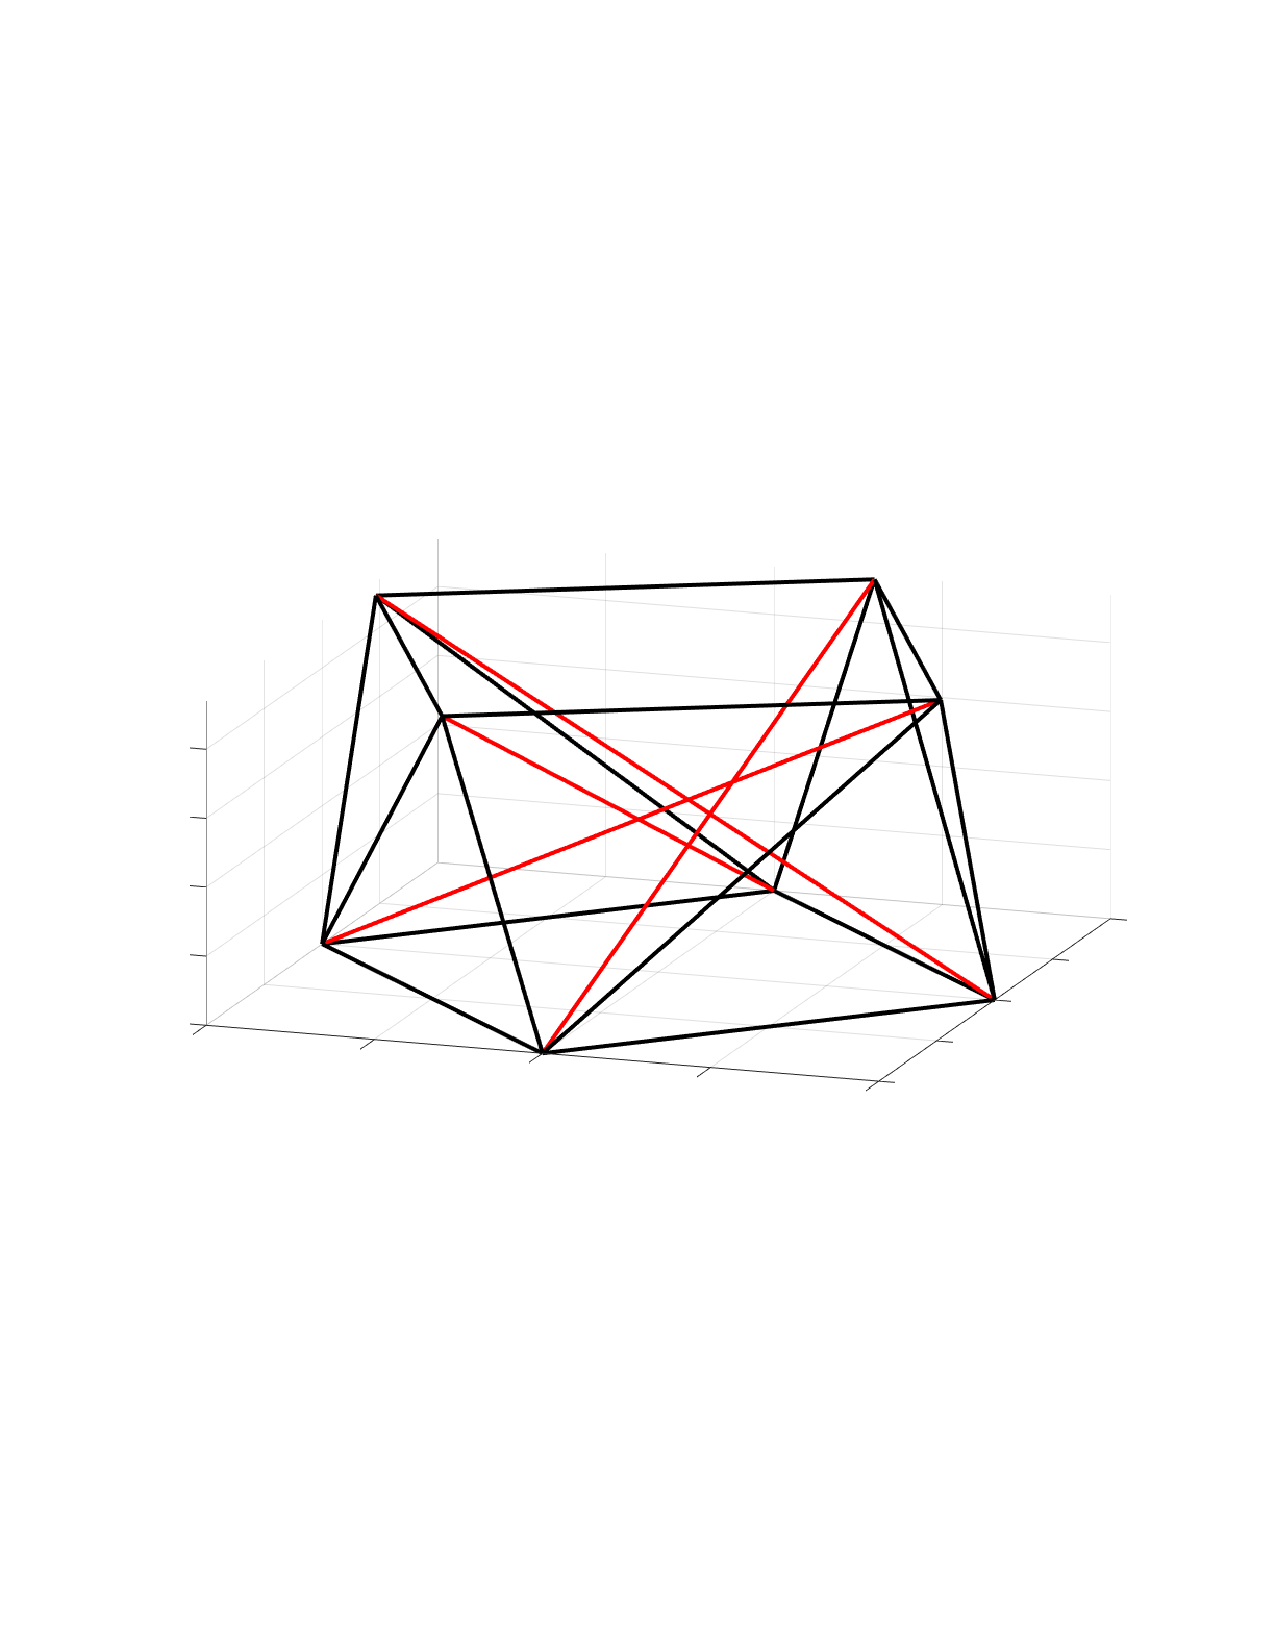
\includegraphics[clip, trim=3.5cm 7.5cm 2.5cm 7.5cm, width=0.6\textwidth]{images/nonminimal_prism_4.pdf}
  \caption{Regular nonminimal prism with 4 bars and 16 strings; bars shown in red, strings shown in black}
  \label{fig:np}
\end{figure}

Ase is potentially inconsistent, implying the presence of soft modes,
or instability!  More strings or fixed points should fix the problem.

Ase is underdetermined with 3 DOF.

Pretensionable!

% Look at the tensions in the strings. There should only be 1 DOF.

\section{Code Output}

\begin{lstlisting}[caption={Ouput of MitchellTruss4.m},captionpos=t, label={lst:p1}]
mhat =

    20


nhat =

    20


r =

    20

Ase is not potentially inconsistent. Good.
 
Bar compressions and string tensions with loads as specified,
least squares solution (i.e., NO pretensioning):

c_bars =

    1.0000    1.0934    1.1956    0.2253    0.2971    0.2463    1.3073    0.3803    0.3362    0.2693

No bars under tension.  Good.

t_strings =

    1.0000    1.0934    1.1956    1.3073    0.2253    0.2971    0.3803    0.2463    0.3362    0.2693

The 10 strings are all under tension with tau_min=0.22527. Good.
 
Ase is not underdetermined (thus, it is not tensionable). The above solution is unique.
\end{lstlisting}


\begin{lstlisting}[caption={Ouput of NonminimalPrism4.m},captionpos=t, label={lst:p2}]
mhat =

    24


nhat =

    20


r =

    17

Warning: Ase is potentially inconsistent, implying the presence of soft modes,
or instability!  More strings or fixed points should fix the problem.
 
Bar compressions and string tensions with loads as specified,
least squares solution (i.e., NO pretensioning):
u in column space of Ase, so at least one solution exists, with residual 0.

c_bars =

     0     0     0     0

No bars under tension.  Good.

t_strings =

     0     0     0     0     0     0     0     0     0     0     0     0     0     0     0     0

Some strings not under tension. Needs different tensioning or external loads.
 
Ase is underdetermined with 3 DOF. Checking now to see if system is pretensionable,
with tension >= 0.1 in all tethers for zero applied load.
 
Result with external load ZERO, pretensioned with given tau_min
while minimizing the L1 norm of the tensions:

c_bars =

    0.4406    0.4406    0.4406    0.4406

No bars under tension.  Good.

t_strings =

  Columns 1 through 10

    0.2253    0.2253    0.2253    0.2253    0.2253    0.2253    0.2253    0.2253    0.1511    0.1511

  Columns 11 through 16

    0.1511    0.1511    0.1000    0.1000    0.1000    0.1000

The 16 strings are all under tension with tau_min=0.1. Good.
 
Pretensionable!
Results with external forces u as specified and tensioned with given tau_min
while minimizing the L1 norm of the tensions.

c_bars =

    0.4406    0.4406    0.4406    0.4406

No bars under tension.  Good.

t_strings =

  Columns 1 through 10

    0.2253    0.2253    0.2253    0.2253    0.2253    0.2253    0.2253    0.2253    0.1511    0.1511

  Columns 11 through 16

    0.1511    0.1511    0.1000    0.1000    0.1000    0.1000

The 16 strings are all under tension with tau_min=0.1. Good.
\end{lstlisting}

\end{document}
